\chapter{Principe d'action de Schwinger}%IV
%43
\section{Introduction}%A
Dans les chapitres précédents, nous avons donné un énoncé
des postulats de Feynman de la mécanique quantique et montré comment
les notions de fonction d'onde, d'équation d'onde et d'opérateurs s'en
déduisaient simplement. Rappelons seulement que nous avons défini l'amplitude de probabilité $<$ x''t'' $|$ x't' $>$ par la relation
\[
\tag{1}<\mt{ x''t'' }|\mt{ x't' }>\ =\sum_\mt{H}\mt{ N exp }\frac{\mt{i}}{\hbar}\mt{ S}_\mt{H}
\]
et l'élément de matrice d'un opérateur G associé à la grandeur classique
g par
\[
\tag{2}\subset \mt{x''t'' }|\mt{ G }|\mt{ x't'}\supset\ =
\sum_\mt{H}\mt{ N g}_\mt{H}\mt{ exp }\frac{\mt{i}}{\hbar}\mt{ S}_\mt{H}
\]
Une telle formulation correspond à une interprétation physique très claire,
en termes d'expériences d'interférence et de diffraction dans l'espace-tenps,
mais conduit en pénéral à des calculs très compliqués.

Nous abordons ici le problème sous un angle nouveau en calculant
la variation $\delta<$ x''t'' $|$ x't' $>$ de l'amplitude de probabilité $<$ x''t'' $|$ x't' $>$
pour des variations infinitésimales de x', t' et x'', t''. Nous donnons tout
d'abord le principe du calcul (\S 2), ce qui nous permet de le rattacher
au problème de la variation de l'action classique que nous traitons ensuite
(\S 3). Nous trouvons alors une expression de $\delta<$ x''t'' $|$ x't' $>$ qui nous
permet d'établir des équations de Lagrange entre opérateurs (\S 4), de définir
l'opérateur d'impulsion P (\S 5) et l'opérateur hamiltonien $\mc{H}$(\S 6).

Si le calcul de $<$ x''t'' $|$ x't' $>$ est assez compliqué, nous allons
voir que celui de $\delta<$ x''t'' $|$ x't' $>$ est beaucoup plus simple et conduit à
une introduction élégante et naturelle des relations de commutations, de
l'équation de Schrödinger, etc.

%44

\section{Princine du calcul de $\delta<$ x''t'' $|$ x't' $>$}%B

\begin{center} 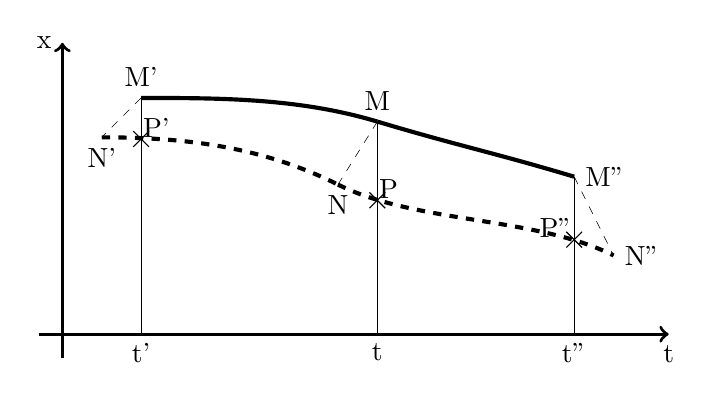
\begin{tikzpicture}
% axes
\draw [->, very thick] (-0.3,0) --++ (8,0) node [below] {t};
\draw [->, very thick] (0,-0.3) --++ (0,4) node [left] {x};
% Chemins
\draw [line width=1.5pt] (1,3) node [above]{M'} .. controls +(1,0) and +(-1,0.3) .. (4,2.7);
\draw [line width=1.5pt] (4,2.7) node [above]{M} .. controls +(1,-0.3) and +(-1,0.3) .. (6.5,2) node [right]{M''};
\draw [line width=1.5pt, dashed] (0.5,2.5) node [below]{N'} .. controls +(1,0) and +(-1,0.5) .. (3.5,1.9);
\draw [line width=1.5pt, dashed] (3.5,1.9) node [below]{N} .. controls +(1,-0.5) and +(-1,0.5) .. (7,1) node [right]{N''};
% abscisses
\draw [very thin] (1,0) node [below] {t'} -- (1,3);
\draw [very thin] (4,0) node [below] {t} -- (4,2.7);
\draw [very thin] (6.5,0) node [below] {t''} -- (6.5,2);
% déplacements
\draw [very thin, dashed] (1,3) -- (0.5,2.5);
\draw [very thin, dashed] (4,2.7) -- (3.5,1.9);
\draw [very thin, dashed] (6.5,2) -- (7,1);
% points
\draw (1.1,2.58)  --(0.9,2.38) node [above right]{P'};
\draw (1.1,2.38) -- (0.9,2.58);
\draw (4.1,1.8) -- (3.9,1.6) node [above right]{P};
\draw (4.1,1.6) -- (3.9,1.8);
\draw (6.6,1.3) -- (6.4,1.1);
\draw (6.4,1.3) -- (6.6,1.1) node [above left]{P''};
\end{tikzpicture} \end{center}
Il s'agit de calculer la quantité
\begin{center}
$\delta<$ x''t'' $|$ x't' $>=<$ x''+$\delta$x'',t''+$\delta$t'' $|$ x'+$\delta$x',t'+$\delta$t' $>-<$ x''t'' $|$ x't' $>$
\end{center}
$\delta$x'',$\delta$t'' et $\delta$x',$\delta$t' représentant la variation infinitésimale la plus
générale des points d'espace-temps M' et M'' qui se trouvent déplacés
en N' et N''.

Le principe du calcul est d'associer à chaque chemin H joignant
M' à M'' (en trait plein sur la figure) un chemin \ul{H} joignent N' à N'' (en
trait pointillé). Pour cela on se donne deux fonctions continues infinitésimales du temps $\delta$x(t) et $\delta$t(t), assujetties aux conditions aux limites.
\[
\tag{3}\left\{ \begin{array}{c}
 \delta\mt{x(t')}=\delta\mt{x'} \\
 \delta\mt{t(t')}=\delta\mt{t'} \\ \end{array} \right.
\left\{ \begin{array}{c}
 \delta\mt{x(t'')}=\delta\mt{x''} \\
 \delta\mt{t(t'')}=\delta\mt{t''} \\ \end{array} \right.
\]
A chaque point M(x, t) d'un chemin M'M'', on associe ainsi un point
N$[$ x+$\delta$x(t), t+$\delta$t(t) $]$. A M' correspond N' et à M'', N''. Ainsi à
tout chemin reliant M' à M'' correspond un chemin relient N' à N'' et réciproquement. Insistons sur le fait que les fonctions $\delta$x(t) et $\delta$t(t) sont
des fonctions de t ne dépendant pas de l'histoire H.

Appelons maintenant S$_\mt{H}$, l'action pour l'histoire H, S$_{\ul{\mt{H}}}$=S$_\mt{H}+\delta$S$_\mt{H}$
l'action pour l'histoire \ul{H}.

%45
Nous avons, d'après la relation (1)
\[
<\mt{ x''t'' }|\mt{ x't' }>\ =\sum_\mt{H}\mt{ N exp }\frac{\mt{i}}{\hbar}\mt{ S}_\mt{H}
\]
\[
<\mt{x''}+\delta\mt{x'',t''}+\delta\mt{t''}|\mt{x'}+\delta\mt{x',t'}+\delta\mt{t'}>=
\sum_{\ul{\mt{H}}}\mt{ N exp }\frac{\mt{i}}{\hbar}\mt{ S}_{\ul{\mt{H}}}=
\sum_\mt{H}\mt{ N exp }\frac{\mt{i}}{\hbar}\mt{ S}_\mt{H}\mt{ exp }\frac{\mt{i}}{\hbar}\ \delta\mt{S}_\mt{H}
\]
Nous pouvons déveloprer au premier ordre exp $\frac{\mt{i}}{\hbar}\ \delta$S$_H=1+\frac{\mt{i}}{\hbar}\ \delta$S$_H$

Il vient alors, par simple soustraction
\[
\tag{4}\delta<\mt{ x''t'' }|\mt{ x't' }>\ =
\frac{\mt{i}}{\hbar}\sum_\mt{H}\mt{ N }\delta\mt{S}_\mt{H}\mt{ exp }\frac{\mt{i}}{\hbar}\mt{ S}_\mt{H}
\]
Si $\mc{S}$ est l'opérateur correspondant à l'action classique (formule (13) du

chapitre III), la relation (4) s'écrit
\[
\tag{5}\delta<\mt{x''t'' }|\mt{ x't'}>\ =
\frac{\mt{i}}{\hbar}\subset \mt{x''t'' }|\ \delta\mc{S}\ |\mt{ x't'}\supset
\]
Sous la forme différentielle (5), la formulation de Feynman constitue le
\ul{Principe d'Action de} \ul{Schwinger}. Pour expliciter cette formule (5), nous
sommes amenés à calculer la variation $\delta\mt{S}_\mt{H}$ de l'action classique le long
de l'histoire H, pour des variations infinitésimales du chemin \ul{et} des
extrémités.

\section{Variation de l'action classique : Calcul de $\delta$S$_\mt{H}$ et Principe d'Action de Schwinger}%C
Soit P le point du chemin \ul{H} correspondant au même temps que M.
Les coordonnées de M sont x, t, celles de N sont x + $\delta$x(t) et t + $\delta$t(t),
celles de P sont x + $\Delta$x$_\mt{H}$(t) et t.

%46
Il est évident que $\Delta$x$_\mt{H}$(t) est différent de $\delta$x(t) et qu'au premier
ordre, on a :
\[
\tag{6}\Delta\mt{x}_\mt{H}=\delta\mt{x(t)}-\dot{\mt{x}}_\mt{H}\mt{(t)}\ \delta\mt{t(t)}
\]
(On voit immédiatement sur la relation (6) qu'alors que $\delta$x(t) est indépendant
de H, $\Delta$x$_\mt{H}$(t) en dépend ( par l'intermédiaire de $\dot{\mt{x}}_\mt{H}$(t) ). C'est ce qui justifie l'indice H dans la notation $\Delta$x$_\mt{H}$(t).

On comprend d'autre part qu'il a été nécessaire d'introduire les deux variations indépendantes $\delta$x(t) et $\delta$t(t), au lieu d'une seule variation $\Delta$x$_\mt{H}$(t),
de façon à pouvoir varier dans le temps les extrémités du chemin H.)

Soient de même P' et P'' les points du chemin \ul{H} aux instants t' et t''.
S$_{\ul{\mt{H}}}$ s'écrit alors sous forme d'intégrale curviligne :
\[
\tag{7}\mt{S}_{\ul{\mt{H}}}=\oint^\mt{N''}_\mt{N'}\mt{L}_{\ul{\mt{H}}}\mt{(t) dt} =
=\oint^\mt{P'}_\mt{N'}\mt{L}_{\ul{\mt{H}}}\mt{ dt}
+\oint^\mt{P''}_\mt{P'}\mt{L}_{\ul{\mt{H}}}\mt{ dt}
+\oint^\mt{N''}_\mt{P''}\mt{L}_{\ul{\mt{H}}}\mt{ dt}
\]
L$_{\ul{\mt{H}}}$(t) étant le lagrangien classique à l'instant t pour l'histoire \ul{H}.
Nous allons évaluer successivement les différents termes de la formule (7) :
\[
\tag{8}\oint^\mt{P'}_\mt{N'}\mt{L}_{\ul{\mt{H}}}\mt{ dt}\simeq
-\delta\mt{t(t') L}_{\ul{\mt{H}}}\mt{(P')}=-\delta\mt{t' L}_{\ul{\mt{H}}}\mt{(P')}\simeq
-\delta\mt{t' L}_{\ul{\mt{H}}}\mt{(M')}=-\delta\mt{t' L}_{\ul{\mt{H}}}\mt{(t')}
\]
De même
\[
\tag{9}\int^\mt{N''}_\mt{P''}\mt{L}_{\ul{\mt{H}}}\mt{ dt}\simeq
\delta\mt{t'' L}_\mt{H}\mt{(t'')}
\]
Les approximations que nous avons faites, qui reviennent à remplacer L$_{\ul{\mt{H}}}$(t)
par la constante L$_\mt{H}$(t'), lagrangien relatif au chemin H à l'instant t', sont
justifiées car nous cherchons une expression au premier ordre.

%47
Enfin
\[
\tag{10}\oint^\mt{P''}_\mt{P'}\mt{L}_{\ul{\mt{H}}}\mt{ dt}=
\int^\mt{t''}_\mt{t'}\mt{L}[\mt{ x}_\mt{H}\mt{(t)}+\Delta\mt{x}_\mt{H}\mt{(t), }
\dot{\mt{x}}_\mt{H}\mt{(t)}+\Delta\dot{\mt{x}}_\mt{H}\mt{(t), t }]\mt{ dt}
\]
Notons que $\dot{\mt{x}}_\mt{H}$(t)+$\Delta\dot{\mt{x}}_\mt{H}$(t) représente la vitesse au point P, égale à
$\frac{\mt{d}}{\mt{dt}}[\mt{x}_\mt{H}$(t)+$\Delta\mt{x}_\mt{H}$(t)] et qu'il en résulte la relation évidente
$\Delta\dot{\mt{x}}_\mt{H}$(t) = $\frac{\mt{d}}{\mt{dt}}\Delta\mt{x}_\mt{H}$(t).

En regroupant les relations (8), (9) et (10) et en soustrayant
\[
\mt{S}_\mt{H}=
\int^\mt{t''}_\mt{t'}\mt{L }[\mt{ x}_\mt{H}\mt{(t)},
\dot{\mt{x}}_\mt{H}\mt{(t) }]\mt{ dt,}
\]
il vient
\[
\tag{11}\delta\mt{S}_\mt{H}=-\delta\mt{t' }\mt{L}_\mt{H}\mt{(t')}+\delta\mt{t'' }\mt{L}_\mt{H}\mt{(t'')}+
\int^\mt{t''}_\mt{t'}\mt{L}[\mt{ x}_\mt{H}+\Delta\mt{x}_\mt{H}\mt{, }
\dot{\mt{x}}_\mt{H}+\Delta\dot{\mt{x}}_\mt{H}\mt{, t }]\mt{ dt}
\]
\[-
\int^\mt{t''}_\mt{t'}\mt{L }[\mt{ x}_\mt{H},
\dot{\mt{x}}_\mt{H}\mt{, t }]\mt{ dt}
\]
En développant les deux derniers termes jusqu'au premier ordre en $\Delta$x$_\mt{H}$ et $\Delta\dot{\mt{x}}_\mt{H}$
il vient
\[
\int^\mt{t''}_\mt{t'}\mt{L}[\mt{ x}_\mt{H}+\Delta\mt{x}_\mt{H}\mt{, }
\dot{\mt{x}}_\mt{H}+\Delta\dot{\mt{x}}_\mt{H}\mt{, t }]\mt{ dt}
-\int^\mt{t''}_\mt{t'}\mt{L }[\mt{ x}_\mt{H},
\dot{\mt{x}}_\mt{H}\mt{, t }]\mt{ dt}
\]
\[
=\int^\mt{t''}_\mt{t'}(\Delta\mt{x}_\mt{H}\frac{\partial\mt{L}}{\partial\mt{x}_\mt{H}}
+\Delta\dot{\mt{x}}_\mt{H}\frac{\partial\mt{L}}{\partial\dot{\mt{x}}_\mt{H}})\mt{ dt}
\]
\[
=\int^\mt{t''}_\mt{t'}\left[\Delta\mt{x}_\mt{H}\frac{\partial\mt{L}}{\partial\mt{x}_\mt{H}}
+(\frac{\mt{d}}{\mt{dt}}\Delta\mt{x}_\mt{H})\frac{\partial\mt{L}}{\partial\dot{\mt{x}}_\mt{H}}\right]\mt{ dt}
\]
%48
et après une intégration par parties élémentaires :
\[
\tag{12}\int^\mt{t''}_\mt{t'}\mt{L }[\mt{ x}_\mt{H}+\Delta\mt{x}_\mt{H}\mt{, }
\dot{\mt{x}}_\mt{H}+\Delta\dot{\mt{x}}_\mt{H}\mt{, t }]\mt{ dt}
-\int^\mt{t''}_\mt{t'}\mt{L }[\mt{ x}_\mt{H},
\dot{\mt{x}}_\mt{H}\mt{, t }]\mt{ dt}
\]
\[
=\Delta\mt{x}_\mt{H}\mt{(t'')}\frac{\partial\mt{L}}{\partial\dot{\mt{x}}_\mt{H}}\mt{(t'')}
-\Delta\mt{x}_\mt{H}\mt{(t')}\frac{\partial\mt{L}}{\partial\dot{\mt{x}}_\mt{H}}\mt{(t')}
+\int^\mt{t''}_\mt{t'}\Delta\mt{x}_\mt{H}\left[\frac{\partial\mt{L}}{\partial\mt{x}_\mt{H}}
-\frac{\mt{d}}{\mt{dt}}\frac{\partial\mt{L}}{\partial\dot{\mt{x}}_\mt{H}}\right]\mt{ dt}
\]
\[
=\mt{p}_\mt{H}\mt{(t'')}\Delta\mt{x}_\mt{H}\mt{(t'')} 
-\mt{p}_\mt{H}\mt{(t')}\Delta\mt{x}_\mt{H}\mt{(t')}
+\int^\mt{t''}_\mt{t'}\Delta\mt{x}_\mt{H}\left[\frac{\partial\mt{L}}{\partial\mt{x}_\mt{H}}
-\frac{\mt{d}}{\mt{dt}}\frac{\partial\mt{L}}{\partial\dot{\mt{x}}_\mt{H}}\right]\mt{ dt}
\]
p$_\mt{H}$(t)$=\frac{\partial\mt{L}}{\partial\dot{\mt{x}}_\mt{H}}$(t) est le moment conjugué de x.

Finalement, compte tenu de (12), (11) devient
\[
\tag{13}\delta\mt{S}_\mt{H}=\int^\mt{t''}_\mt{t'}\Delta\mt{x}_\mt{H}(\frac{\partial\mt{L}}{\partial\mt{x}_\mt{H}}
-\frac{\mt{d}}{\mt{dt}}\frac{\partial\mt{L}}{\partial\dot{\mt{x}}_\mt{H}})\mt{ dt}
+\mt{L}_\mt{H}\mt{(t'') }\delta\mt{t''}+\mt{p}_\mt{H}\mt{(t'') }\Delta\mt{x}_\mt{H}\mt{(t'')}
\]
\[
-\mt{L}_\mt{H}\mt{(t') }\delta\mt{t'}-\mt{p}_\mt{H}\mt{(t') }\Delta\mt{x}_\mt{H}\mt{(t')}
\]
On peut maintenant éliminer $\Delta$x$_\mt{H}$ en utilisant la relation (6).
On introduit alors la fonction hamiltonienne H$_\mt{H}$(t) = P$_\mt{H}$(t) $\dot{\mt{x}}_\mt{H}$(t) - L$_\mt{H}$(t)
et (13) devient
\[
\tag{14}\delta\mt{S}_\mt{H}=\int^\mt{t''}_\mt{t'}(\delta\mt{x(t)}-\dot{\mt{x}}_\mt{H}\mt{(t) }\delta\mt{t(t)})
\left(\frac{\partial\mt{L}}{\partial\mt{x}_\mt{H}}
-\frac{\mt{d}}{\mt{dt}}\frac{\partial\mt{L}}{\partial\dot{\mt{x}}_\mt{H}}\right)\mt{ dt}
\]
\[
-\mt{H}_\mt{H}\mt{(t'') }\delta\mt{t''}+\mt{p}_\mt{H}\mt{(t'') }\delta\mt{x''}
+\mt{H}_\mt{H}\mt{(t') }\delta\mt{t'}-\mt{p}_\mt{H}\mt{(t') }\delta\mt{x'}
\]
Remarques :

— Le calcul précédent est un calcul de base de mécanique analytique \ul{classique}.
Il montre notamment comment s'introduisent de façon naturelle les notions de
moment conjugué et de hamiltonien.

— Si on pose $\delta$x' = $\delta$x'' = $\delta$t' = $\delta$t'' = 0, la variation de l'action $\delta$S$_\mt{H}$ se
réduit à $\int^\mt{t''}_\mt{t'}\Delta\mt{x}_\mt{H}(\frac{\partial\mt{L}}{\partial\mt{x}_\mt{H}}-\frac{\mt{d}}{\mt{dt}}\frac{\partial\mt{L}}{\partial\dot{\mt{x}}_\mt{H}})$dt. Si on postule que le chemin classique
%49
entre M' et M'' est le chemin d'action stationnaire, la trajectoire
classique x$_\mt{C}$(t) doit être telle que $\delta$S$_\mt{H}$ est nul $\forall\Delta$x(t), et on retrouve alors les équations de Lagrange $\frac{\partial\mt{L}}{\partial\mt{x}_\mt{C}}-\frac{\mt{d}}{\mt{dt}}\frac{\partial\mt{L}}{\partial\dot{\mt{x}}_\mt{C}}=0$

Cependant, pour une histoire H \ul{quelconque}, l'intégrale $\int^\mt{t''}_\mt{t'}(\frac{\partial\mt{L}}{\partial\mt{x}_\mt{H}}-\frac{\mt{d}}{\mt{dt}}\frac{\partial\mt{L}}{\partial\dot{\mt{x}}_\mt{H}})\Delta$x$_\mt{H}$
 dt n'est pas nulle et doit, en conséquence,
figurer dens l'expression (14).

La relation (14) est une relation de la mécanique classique,
entre grandeurs classiques.

Cependant, nous avons vu (chapitre III) que le formalisme de
Feynman permet d'associer à toute grandeur classique g$_\mt{H}$ un orérateur
quantique G par la relation (2). Ainsi, à x$_\mt{H}$(t) on associe l'opérateur
X(t), à $\dot{\mt{x}}_\mt{H}$(t) l'opérateur $\dot{\mt{X}}$(t), à L(x$_\mt{H}$, $\dot{\mt{x}}_\mt{H}$) l'opérateur $\mc{L}$(X, $\dot{\mt{X}}$),
à p = $\frac{\partial\mt{L}}{\partial\dot{\mt{x}}}$ l'opérateur P = $\frac{\partial\mc{L}}{\partial\dot{\mt{X}}}$ et enfin au hamiltonien H $=\mt{p}_\mt{H}\dot{\mt{x}}_\mt{H}-\mt{L}_\mt{H}$,
l'opérateur $\mc{H}=\mt{P}\dot{\mt{X}}-\mc{L}(\mt{X},\dot{\mt{X}})$.

La relation (14) se transcrit immédiatement aux opérateurs en
raison de la linéarité de la relation (2) et compte tenu de (5), il vient
\[
\tag{15}\delta<\mt{ x''t'' }|\mt{ x't' }>\ =\ 
<\mt{x''+}\delta \mt{x'', t''}+\delta \mt{t'' }|\mt{ x'}+\delta \mt{x', t'}+\delta \mt{t'}> - <\mt{ x''t'' }|\mt{ x't' }>
\]
\[
=\frac{\mt{i}}{\hbar}\subset \mt{x''t'' }|\ \delta\mt{S}\ |\mt{ x't'}\supset
\]
\[
=\frac{\mt{i}}{\hbar}\subset \mt{x''t'' }|\mt{ P(t'')}\delta\mt{x''}-\mt{ P(t')}\delta\mt{x'}
-\mc{H}\mt{(t'')}\delta\mt{t''}+\mc{H}\mt{(t')}\delta\mt{t'}\ |\mt{ x't'}\supset
\]
\[
+\frac{\mt{i}}{\hbar}\subset \mt{x''t'' }
\int^\mt{t''}_\mt{t'}
\left(\frac{\partial\mc{L}}{\partial\mt{X}}
-\frac{\mt{d}}{\mt{dt}}\frac{\partial\mc{L}}{\partial\dot{\mt{X}}_\mt{H}}\right)
\left[\delta\mt{x(t) I}-\delta\mt{t(t)}\dot{\mt{X}}\mt{(t)}\right]\mt{dt}\ |\mt{ x't'}\supset
\]

La formule (15) qui traduit le \ul{Principe d'Action de Schwinger}
va constituer le point de départ de notre étude. Elle appelle quelques
remarques :

%50
$\alpha$) $\delta$x(t) ne dépendant pas de H, l'élément de matrice
$\sum_\mt{H}(\mt{exp}\frac{\mt{i}}{\hbar}$ S$_\mt{H})\delta$x(t)
se factorise et s'écrit $\delta\mt{x(t)}\subset \mt{x''t'' }|\mt{ I }|\mt{ x't'}\supset$, I étant l'opérateur identité,
$\delta$x(t) doit donc être considéré comme un nombre, ou ce qui revient au mêre,
comme un multiple de la matrice unité. C'est ce qui explique l'introduction
de la matrice unité I dans le deuxième terme de la relation (15).

$\beta$) La notion d'intégrale d'opérateur introduite dans le deuxième terme de
(15) peut se comprendre comme une intégrale au sens de Riemam, limite d'une
somme d'opérateurs pris à des instants infiniment voisins entre t' et t''.


\section{Equations de Lagrange en mécanique quantique}%D
Faisons tout d'abord l'hypothèse que la variation aux bornes est
nulle : $\delta$x' = $\delta$x'' = $\delta$t' = $\delta$t'' = 0. N' est confondu avec M', N'' avec M''.
H et \ul{H} représentent alors deux chemins infiniment voisins passant tous
deux par les points M' et M''. Pour passer de l'un à l'autre, on se donne
les deux fonctions infinitésimales $\delta$x(t) et $\delta$t(t). Mais, dans ce cas particulier, il est inutile d'introduire deux variations indépendantes et on peut
poser $\delta$t(t) $\equiv$ 0, La correspondance est donc assurée à l'aide de la fonction
infinitésimale $\delta$x(t), identique pour tous les chemins H, obéissant aux relations $\delta$x(t') = $\delta$x(t'') = 0 et à part cela arbitraire.

Comme à tout chemin H correspond un chemin \ul{H} et réciproquement
et que les points de départ et d'arrivée sont les mêmes, on a évidemment
\[
\tag{16}\sum_\mt{H}\mt{N exp}\frac{\mt{i}}{\hbar}\mt{S}_\mt{H}=
\sum_\mt{\ul{H}}\mt{N exp}\frac{\mt{i}}{\hbar}\mt{S}_\mt{\ul{H}}
\]
le passage de l'un à l'autre de ces expressions revenant à effectuer un
changement d'indice "muet" H.

On déduit de (16) que $\delta$ < x''t''|x't' > = 0, ce qui, compte tenu
de (15), conduit à
\[
\tag{17}\subset \mt{x''t'' }|
\int^\mt{t''}_\mt{t'}
\left[\frac{\partial\mc{L}}{\partial\mt{X}}
-\frac{\mt{d}}{\mt{dt}}\frac{\partial\mc{L}}{\partial\dot{\mt{X}}}\right]
\delta\mt{x(t) }\mt{dt}\ |\mt{ x't'}\supset=0
\]

%51
La relation (17) est vraie quelle que soit la fonction infinitésimale $\delta$x(t)
satisfaisant aux conditions $\delta$x(t') $= \delta$x(t'') $=$ 0,
Choisissons pour $\delta$x(t) une fonction nulle partout, sauf dans un intervalle
très petit autour de t. Pour que (17) soit satisfaite, il faut que l'on ait :
\[
\subset \mt{x''t'' }|
\left[\frac{\partial\mc{L}[\mt{X(t), }\dot{\mt{X}}\mt{(t), t}]}{\partial\mt{[X(t)}]}
-\frac{\mt{d}}{\mt{dt}}\frac{\partial\mc{L}[\mt{X(t), }\dot{\mt{X}}\mt{(t), t}]}{\partial\dot{\mt{X}}\mt{(t)}}\right]
|\mt{ x't'}\supset=0
\]
ce qui nous conduit à la relation entre opérateurs :
\[
\tag{18}\frac{\partial\mc{L}}{\partial\mt{X}}\mt{(t)}
-\frac{\mt{d}}{\mt{dt}}\frac{\partial\mc{L}}{\partial\dot{\mt{X}}}\mt{(t)}=0\ \ \ \ \ \ (\forall\mt{t})
\]

La relation (18) est la généralisation aux opérateurs quantiques
des équations de Lagrange classiques, Elle a été déduite directement des
postulats de Feynman, ou ce qui revient au même, du Principe d'Action de
Schwinger. Elle est valable quel que soit $\hbar$ et non pas seulement à la
limite classique.

Les opérateurs qui interviennent dans cette équation de Lagrange
étant des opérateurs à un seul instant t, nous savons (cf chapitre III)
qu'il y a équivalence entre les définitions de Feynmen et de Heisenberg
des opérateurs (à condition d'appliquer la règle de symétrisation).

On retrouve ainsi le fait que dans la représentation de Heisenberg,
les opérateurs satisfont aux équations de le mécanique classique. Prenons en
effet pour exemple le cas d'une particule dans un potentiel V(x). Le lagrangien quantique s'écrit  - V(X) et l'équation (18) conduit à la relation entre onérateurs, au sens de Feynman et de Heisenberg :
\[
\tag{19}\mt{m}\frac{\mt{d}\dot{\mt{X}}}{\mt{dt}}=
-\frac{\partial\mt{V}}{\partial\mt{X}}
\]
qui n'est autre que l'équation fondamentale de la dynamique newtonienne.
Dans le formalisme habituel de Heisenberg, (19) s'établit à partir de
l'équation d'évolution de l'opérateur P :

%52
\[
\tag{20}\mt{i}\hbar=[\mt{P, }\mc{H}]
\]
Or
\[
\tag{21}[\mt{P, }\mc{H}]=-\mt{i}\hbar\frac{\partial\mc{H}}{\partial\mt{X}}=
-\mt{i}\hbar\frac{\partial\mt{V}}{\partial\mt{X}}
\]
(20) et (21) redonnent (19).

Si on prend la moyenne des deux membres de (19) dans un état
| $\psi$ > quelconque, on retrouve le fait que les moyennes quantiques obéissent
aux lois d'évolution des grandeurs classiques correspondantes : c'est le
\ul{théorème d'Ehrenfest}.

Reprenons maintenant la relation fondamentale (15), en tenant
compte du fait que $\frac{\partial\mc{L}}{\partial\mt{X}}
-\frac{\mt{d}}{\mt{dt}}\frac{\partial\mc{L}}{\partial\dot{\mt{X}}}$ est identiquement nul. Il vient :
\[
\tag{22}\delta<\mt{ x''t'' }|\mt{ x't' }>\ =\frac{\mt{i}}{\hbar}\subset \mt{x''t'' }|\ \delta\mt{S}\ |\mt{ x't'}\supset
\]
\[
=\frac{\mt{i}}{\hbar}\subset \mt{x''t'' }|\ \mt{ P(t'')}\delta\mt{x''}-\mt{ P(t')}\delta\mt{x'}
-\mc{H}\mt{(t'')}\delta\mt{t''}+\mc{H}\mt{(t')}\delta\mt{t'}\ |\mt{ x't'}\supset
\]
Chacun des opérateurs de la relation (22) est maintenant un opérateur à
un seul temps et on peut écrire dans le point de vue de Heisenberg :
\[
\tag{23}<\mt{x''+}\delta \mt{x'', t''}+\delta \mt{t'' }|\mt{ x'}+\delta \mt{x', t'}+\delta \mt{t'}> - <\mt{ x''t'' }|\mt{ x't' }>
\]
\[
=\frac{\mt{i}}{\hbar}< \mt{x''t'' }|\ \mt{ P(t'')}\delta\mt{x''}-\mt{ P(t')}\delta\mt{x'}
-\mt{H(t'')}\delta\mt{t''}+\mt{H(t')}\delta\mt{t'}\ |\mt{ x't'}>
\]

\section{Opérateur impulsion : P(t)}%E
Faisons dans la relation (23) $\delta$x''$= \delta$t'$= \delta$t''$= 0;\ \delta$x' $\neq 0$.
On obtient la relation :
\[
\tag{24}<\mt{x'', t'' }|\mt{ x'}+\delta \mt{x', t'}> - <\mt{ x''t'' }|\mt{ x't' }>=-\frac{\mt{i}}{\hbar}\delta\mt{x'}< \mt{x''t'' }|\ \mt{ P(t')}\ |\mt{ x't'}>
\]
La relation (24),étant vraie quel que soit < x''t'' | , entraîne
\[
|\mt{ x'}+\delta \mt{x', t'}>\ =|\mt{ x't' }>-\frac{\mt{i}\delta\mt{x'}}{\hbar}\ \mt{ P(t')}\ |\mt{ x't'}>
\]
%53
Soit
\[
\tag{25}|\mt{ x'}+\delta \mt{x', t'}>\ =\left[1-\frac{\mt{i}\delta\mt{x'}}{\hbar}\ \mt{ P(t')}\right]\ |\mt{ x't'}>
\]
L'opérateur P (t') étant hermitique, 1 - $\frac{\mt{i}\delta\mt{x'}}{\hbar}$ P(t') est un
opérateur unitaire infinitésimal qui translate | x', t' > en | x' + x'', t' >.
P(t), opérateur impulsion, est donc le "générateur" du groupe des translations dans l'espace des états de la mécanique quantique. C'est la propriété
fondamentale de P. A partir de (25), nous pouvons retrouver les différentes
propriétés de l'opérateur P :


\subsubsection{Commutateur [x (t'), P (t')]}%a
D'après (25) :
\[
\mt{P(t')}\ |\mt{ x', t'}>\ =\frac{\mt{i}\hbar}{\delta\mt{x'}}\ 
[\ |\mt{ x'}+\delta \mt{x', t'}>-|\mt{x', t'}>]
\]
et
\[
\mt{X(t') P(t')}\ |\mt{ x', t'}>\ =
\frac{\mt{i}\hbar}{\delta\mt{x'}}\ 
[\ (\mt{ x'}+\delta \mt{x'})|\mt{ x'}+\delta \mt{x', t'}>-
\mt{ x'}|\mt{x', t'}>]
\]
D'autre part
\begin{center}
X(t') $|$ x't' $> =$ x' $|$ x't' $>$

et \ \ \ \ P(t') X(t') $|$ x't' $> = \frac{\mt{i}\hbar}{\delta\mt{x'}}$
$[$ x' $|$ x' $+ \delta$x', t' $> -$ x' $|$ x't'$>]$
\end{center}
Finalement
\begin{center}
$[$ X(t') P(t') - P(t') X(t') $]\ |$ x't' $> = [$ X(t'), P(t') $]\ |$ x't' $> = \mt{i}\hbar |$ x' + $\delta$x', t' >
\end{center}
Cette relation est vérifiée à le limite où $\delta$x' tend vers zéro.
On a donc :
\begin{center}
$[$ X(t'), P(t') $]\ |$ x't' $> = \mt{i}\hbar\ |$ x't' $>$
\end{center}
Les vecteurs | x't' > à t' fixé constituent un ensemble complet.
On en déduit donc :
\[
\tag{26}[\mt{ X(t), P(t) }]=\mt{i}\hbar\ \ \ \ \ \ (\forall\mt{t})
\]
et dans le formalisme de Schrôdinger :
\[
\tag{27}[\ \mt{\ul{X}},\ \mt{\ul{P}}\ ]=\mt{i}\hbar
\]
ce qui constitue la relation de commutation fondamentale des opérateurs
position et impulsion.
%54

\subsection{Opérateur P dans la représentation x}%b

La relation conjuguée de (25) s'écrit :
\[
\tag{28}<\mt{ x}+\delta \mt{x, t }|\ =<\mt{ x, t }|+\frac{\mt{i}\delta\mt{x}}{\hbar}<\mt{ x, t }|\ \mt{ P(t) }
\]
Nous cherchons à déterminer l'action de P(t) sur un état $|\psi>$ défini
par sa fonction d'onde $<$ x, t $|\psi> = \psi$ (x, t), c'est-à-dire qu'à partir
de $\psi$(x, t) nous cherchons la fonction d'onde $\phi$(x, t) $= <$ x, t $|$ P(t) $|\psi>$.
Multiplions (28) membre à membre par $|\psi>$.

Il vient  $\psi$(x + $\delta$x, t) $=\psi$(x, t) $+ \frac{\mt{i}\delta\mt{x}}{\hbar}\phi$(x, t).
Soit  $\phi$(x, t) $=\frac{\hbar}{\mt{i}}\frac{\psi\mt{(x+}\delta\mt{x, t)}-\psi\mt{(x, t)}}{\delta\mt{x}}$

Cette relation n'est vérifiée qu'à la limite où $\delta$x $\to$ 0. On a donc en fait :
\[
\tag{29}\phi\mt{(x,t)}=\frac{\hbar}{\mt{i}}\frac{\partial}{\partial\mt{x}}\psi\mt{(x,t)}
\]
et \ul{en représentation x, l'opérateur P est donc} $\frac{\hbar}{\mt{i}}\frac{\partial}{\partial\mt{x}}$.

 

Le formalisme de Feynman permet ainsi de retrouver de façon
simple les propriétés fondamentales de l'opérateur impulsion P en le rattachant au groupe des opérateurs de translation dans l'espace des états.
\section{Opérateur hamiltonien H (t)}%F
Reprenons maintenant la relation (23) en y faisant
$\delta$x'' $=\delta$x' $=\delta$t'' $= 0$; $\delta$t' $\neq 0$.

On obtient la relation
\[
\tag{30}=
\]
La relation (30) étant vraie, quel que soit < x''t'' | , entraîne

%55
Soit
\[
\tag{31}=
\]
L'opérateur  étant hermitique,  est l'opérateur
infinitésimal unitaire qui translate | x' t' > dans le temps en
| x, t' + t' >.
Le hamiltonien (t) est le générateur du groupe des translations dans le
temps.

A partir de l'équation (31), nous pouvons retrouver l'équation
de Schrôdinger.

La relation conjuguée de (31) s'écrit :

En multipliant membre à membre par un état |  > , on obtient

où, à la limite où t  0 :
\[
\tag{32}=
\]
(32) n'est rien d'autre que l'équation de Schrôdinger en représentation x.
En effet
et (32) s'écrit :
\[
\tag{33}=
\]
Nous retrouvons ainsi, de façon beaucoup plus élégante, l'équation de
Schrôdinger que nous avons déjà déduite directement des postulats de
Feynman au chapitre II.

